\sectionLabel{Problem Representation}

\subsectionLabel{Feature Selection}

A target problem in \textit{\projectTitle{}} consists of:
\begin{enumerate}
    \item A sentence
    \item A target word in that sentence to correct
\end{enumerate}

Both the \textit{Bayesian} and \textit{Winnow-based} algorithms studied here
represent the problem as a list of active features. Each active feature
indicates the presence of a particular linguistic pattern in the context of the
target word.

We use two types of features:
\begin{description}
    \item [Context words:]
        \textit{Context-word} features test for the presence of a particular
        word within \(\pm k\) words of the target word.
    \item [Collocations:]
        \textit{Collocations} test for a pattern of up to \(l\) contiguous words
        and/or part-of-speech tags around the target word.
\end{description}

In the experiments reported here, \(k\) was set to \(10\) and \(l\) was set to
\(2\). Examples of useful features for the confusion set \(\{weather,
whether\}\) include:
\begin{enumerate}
    \item \(cloudy\) within \(\pm 10\) words
    \item \(\text{\ul{~~~~~~~~~~}\ } to \text{\ } VERB\)
\end{enumerate}

Feature (1) is a context-word feature that tends to imply \(weather\). Feature
2 is a collocation that checks for the pattern \textit{``to VERB''} immediately
after the target word, and tends to imply \(whether\) as in \ex(I don't know
whether to laugh to cry).

\subsubsection{Context Words}

One clue about the identity of an ambiguous target word comes from the words
around it. For instance, if the target word is ambiguous between \(desert\) and
\(dessert\), and we see words like \(arid\), \(sand\) and \(sun\) nearby, this
suggests that the target word should be \(desert\). On the other hand, words
such as \(chocolate\) and \(delicious\) in the the context imply \(dessert\).
This observation is the basis for the method of context words. The idea is that
each word \(w_i\) in the confusion set will have a characteristic distributions
of words that occur in its context; thus to classify an ambiguous target word,
we look at the set of words around it and which \(w_i\)'s distribution they
most closely follow. The main parameter to tune for the method of context words
is \(k\), the half-width of the context windows. Previous work
\cite{yarowsky1994decision} shows that smaller values of \(k\) (3 or 4) work
well for resolving local syntactic ambiguities, while larger values (20 to 50)
are suitable for resolving semantic ambiguities. We tried the values \(3\),
\(6\), \(9\), \(10\), \(12\), \(16\), \(18\), \(20\) and \(24\) on our
confusion sets and found that \(k = 10\) worked the best in general cases. In
the rest of the document, this value of \(k\) will be used when referring to
\(k\).
\begin{figure}[H]
\caption{Effect of different values of \(k\) on context words}
\begin{tabularx}{\textwidth}{l R}
    \(k = 10\) & But, \ul{how} I sometimes need a moment of rest, and \emph{peace}\\
    \(k = 8\)  & No matter \ul{how} earnest is out quest for guaranteed \emph{peace}\\
    \(k = 6\)  & \ul{How} best to destroy your \emph{peace}?
\end{tabularx}
\end{figure}

\begin{figure}[H]
    \caption{Outline of the method of using \textit{context words}}
    \ul{Training Phase}\\
    \begin{enumerate}
        \item Propose all words as candidate context words.
        \item Count occurrences of each candidate context word in the training
        corpus.
        \item Prune context words that have insufficient data or are
        uninformative.
        \item Store the remaining context words and their associated statistics
        for use at run time.
    \end{enumerate}
    \vspace{\baselineskip}
    \ul{Run Time}\\
    \begin{enumerate}
        \item Initialize the probability for each word in the confusion set to
        its prior probability.
        \item Go through the list of context words that was saved during
        training. For each context word that appears in the context of the
        ambiguous target word, update the probabilities.
        \item Choose the word in the confusion set with the highest probability.
    \end{enumerate}
    \vspace{\baselineskip}
\end{figure}

\subsubsection{Collocations}

The method of context words is good at capturing generalities that depend on
the presence of nearby words, but not their order. When order matters, other
more syntax-based methods, such as collocations and trigrams, are appropriate.
We used collocations to capture order dependencies. A collocation expresses a
pattern of syntactic elements around the target word. We allow two types of
syntactic elements: words and part-of-speech tags.\\ Going back to the
\(\{desert, dessert\}\) example, a collocation would imply \(desert\) might be:
\begin{center}
    \(PREP \text{\ }the\text{\ \ul{~~~~~~~~~~}}\)
\end{center}

This collocation would match the sentences:
\begin{center}
    Travellers entering from the \ul{\emph{desert}} were confounded\ldots\\
    \ldots along with some guerilla fighting in the \ul{\emph{desert}}.\\
    \ldots two ladies who lay by pinkly beside him in the \ul{\emph{desert}}\ldots
\end{center}

Matching part-of-speech tags against the sentence is done by first tagging each
word in the sentence with its set of possible part-of-speech tags obtained from
a dictionary and a language model. For instance, \(walk\) has the tag set
\(\{NS, V\}\) corresponding to its use as a singular noun and as a verb. For a
tag to match a word, the tag must be a member of the word's tag set. The reason
we use tag sets instead of running a tagger on the sentence to produce unique
tags is that taggers need to look at all the words in the sentence which
doesn't make a lot of sense when the target word in the sentence itself is
ambiguous.

The method of collocations was implemented in much the same way as the method
of context words. The idea is to discriminate among the words \(w_i\) in the
confusion set by identifying the collocations that tend to occur around each
\(w_i\). An ambiguous target word is then classified by finding all
collocations that match its context. Each collocation provides some degree of
evidence for each word in the confusion set.

Like the method of context words, the method of collocations has one main
parameter to tune: \(l\), the maximum number of syntactic elements in a
collocation. Since the collocations grow exponentially with \(l\), we varied
\(l\) from \(1\) to \(3\) and finally settled on \(2\).

\subsectionLabel{Intuition for Feature Selection}

The intuition for using these two types of features is that they capture two
important, but complementary aspects of context. Context words tell us what
kind of words tend to appear in the vicinity of the target word --- the
``lexical atmosphere''. They therefore capture aspects of the context with a
wide-scope, semantic flavour, such as discourse topic and tense. Collocations,
in contrast, capture the local syntax around the target word. Similar
combinations of features have been used in related tasks, such as accent
restoration \cite{yarowsky1994decision} and word-sense disambiguation \cite{ng1996integrating}.\\

\subsectionLabel{Feature Extraction}

We use a \textit{feature extractor} to convert from the initial text
representation of a sentence to a list of active features called a
\textit{feature vector}. The feature extractor has a preprocessing phase in
which learns a set of features for the task. Thereafter, it can convert a
sentence into a list of active features simply by matching its set of learned
features against the sentence.

In the preprocessing phase, the feature extractor learns a set of features that
characterize the contexts in which each word \(w_i\) in the confusion set tends
to occur. This involves going through the training corpus, and, each time a
word in the confusion set occurs, generating all possible features for the
context --- namely, one context-word feature for every distinct word within
\(\pm k\) words, and one collocation for every way of expressing a pattern of
up to \(l\) contiguous elements. This gives an exhaustive list of all features
found in the training set.

\subsectionLabel{Feature Pruning}

Statistics of occurrence of the features are collected in the process as well.
At this point, pruning criteria may be applied to eliminate unreliable or
uninformative features.\\
We use two criteria (which make use of the aforementioned statistics of
occurrence):
\begin{enumerate}
    \item The feature occurred in practically none or all of the training instances (specifically, it had fewer than 10 occurrences or fewer than 10 non-occurrences)
    \item The presence of the feature is not significantly correlated with the identity of the target word (determined by a \textit{chi-square test} at the \(0.05\) significance level).
\end{enumerate}

\begin{figure}[h]
    \centering
    \caption{Prediction of a sentence using Winnow}
    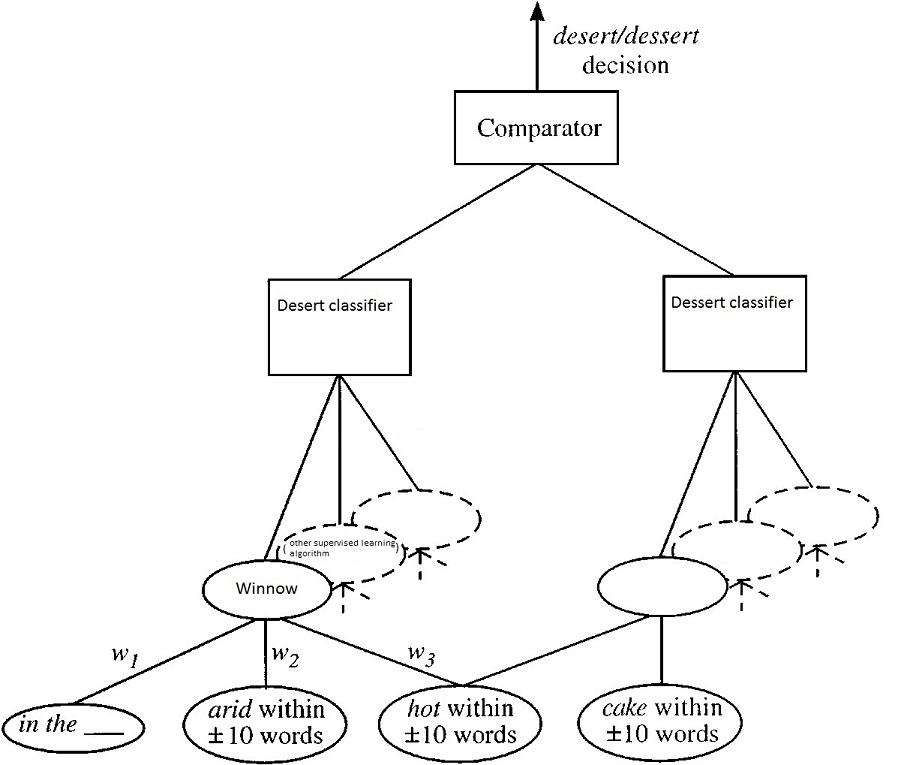
\includegraphics[width=130mm]{img/winnow.jpg}
\end{figure}
\null\vfill
